%\documentclass{standalone}
%\usepackage{tikz}
%\usetikzlibrary{patterns,plotmarks}
%\begin{document}
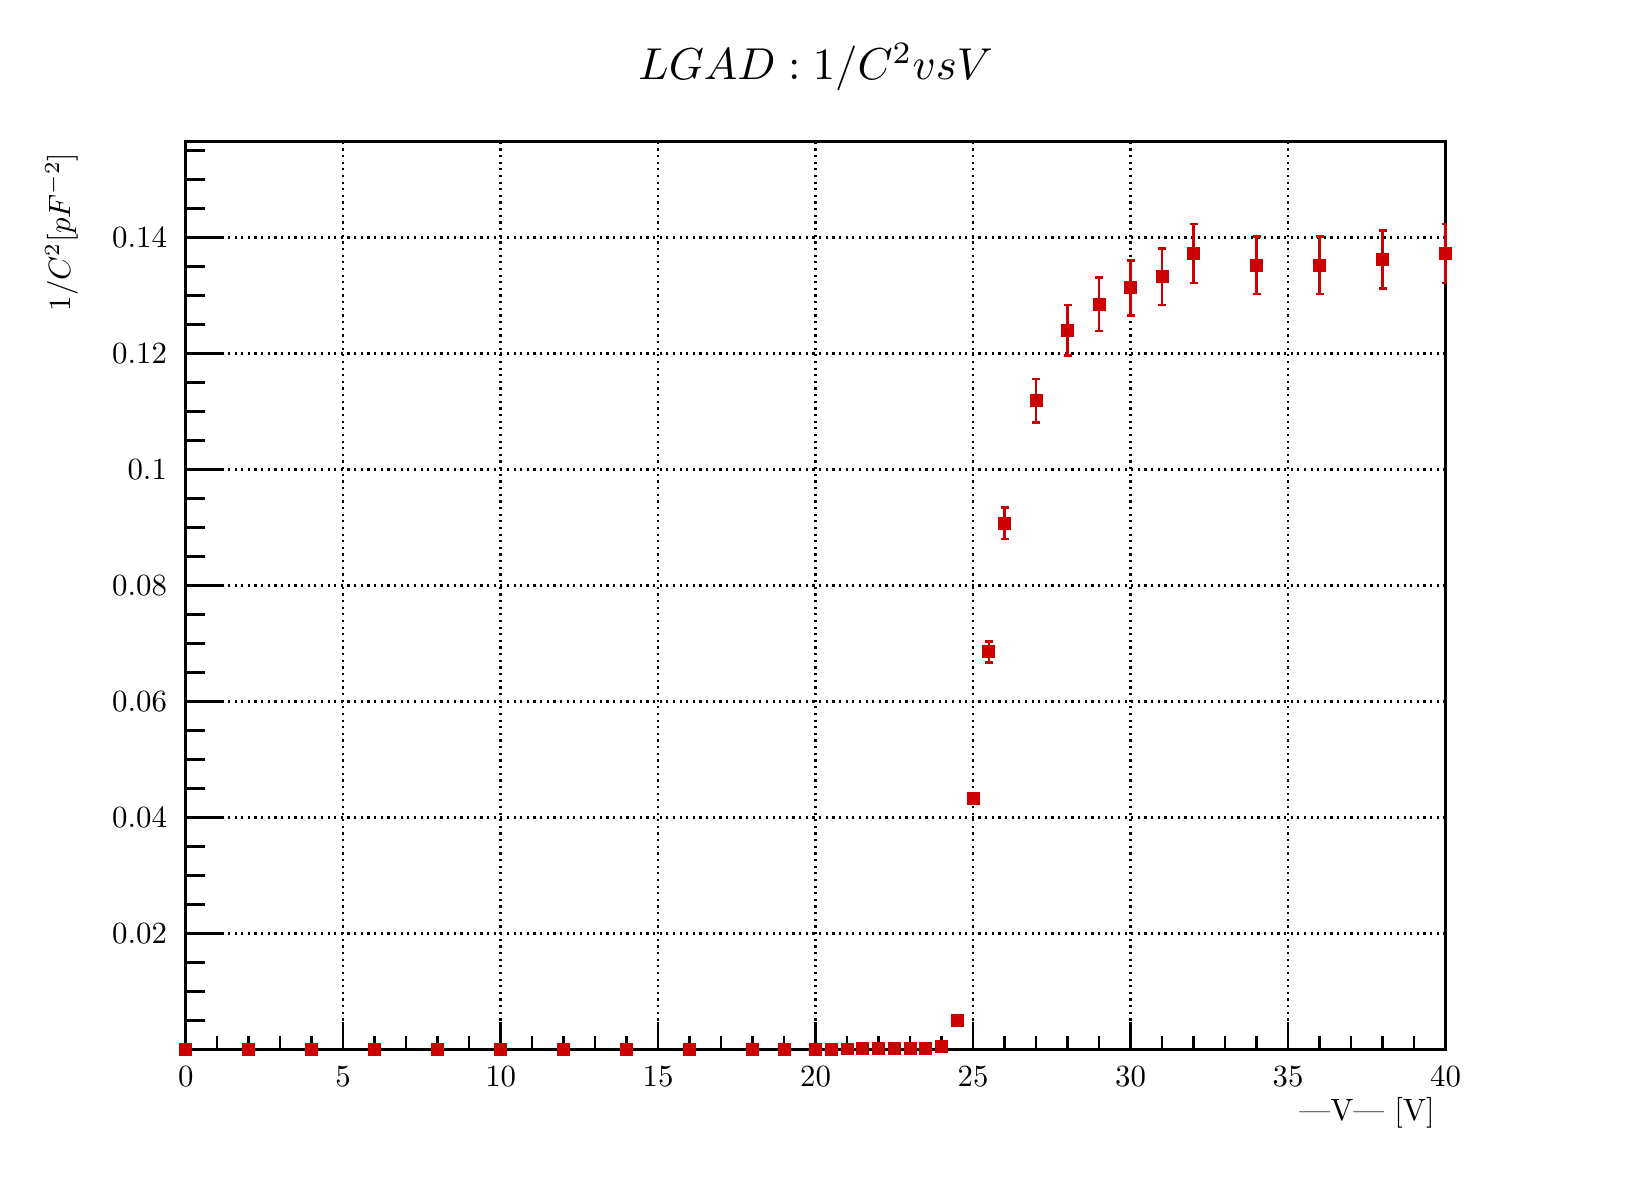
\begin{tikzpicture}
\def\CheckTikzLibraryLoaded#1{ \ifcsname tikz@library@#1@loaded\endcsname \else \PackageWarning{tikz}{usetikzlibrary{#1} is missing in the preamble.} \fi }
\CheckTikzLibraryLoaded{patterns}
\CheckTikzLibraryLoaded{plotmarks}
\pgfdeclareplotmark{cross} {
\pgfpathmoveto{\pgfpoint{-0.3\pgfplotmarksize}{\pgfplotmarksize}}
\pgfpathlineto{\pgfpoint{+0.3\pgfplotmarksize}{\pgfplotmarksize}}
\pgfpathlineto{\pgfpoint{+0.3\pgfplotmarksize}{0.3\pgfplotmarksize}}
\pgfpathlineto{\pgfpoint{+1\pgfplotmarksize}{0.3\pgfplotmarksize}}
\pgfpathlineto{\pgfpoint{+1\pgfplotmarksize}{-0.3\pgfplotmarksize}}
\pgfpathlineto{\pgfpoint{+0.3\pgfplotmarksize}{-0.3\pgfplotmarksize}}
\pgfpathlineto{\pgfpoint{+0.3\pgfplotmarksize}{-1.\pgfplotmarksize}}
\pgfpathlineto{\pgfpoint{-0.3\pgfplotmarksize}{-1.\pgfplotmarksize}}
\pgfpathlineto{\pgfpoint{-0.3\pgfplotmarksize}{-0.3\pgfplotmarksize}}
\pgfpathlineto{\pgfpoint{-1.\pgfplotmarksize}{-0.3\pgfplotmarksize}}
\pgfpathlineto{\pgfpoint{-1.\pgfplotmarksize}{0.3\pgfplotmarksize}}
\pgfpathlineto{\pgfpoint{-0.3\pgfplotmarksize}{0.3\pgfplotmarksize}}
\pgfpathclose
\pgfusepathqstroke
}
\pgfdeclareplotmark{cross*} {
\pgfpathmoveto{\pgfpoint{-0.3\pgfplotmarksize}{\pgfplotmarksize}}
\pgfpathlineto{\pgfpoint{+0.3\pgfplotmarksize}{\pgfplotmarksize}}
\pgfpathlineto{\pgfpoint{+0.3\pgfplotmarksize}{0.3\pgfplotmarksize}}
\pgfpathlineto{\pgfpoint{+1\pgfplotmarksize}{0.3\pgfplotmarksize}}
\pgfpathlineto{\pgfpoint{+1\pgfplotmarksize}{-0.3\pgfplotmarksize}}
\pgfpathlineto{\pgfpoint{+0.3\pgfplotmarksize}{-0.3\pgfplotmarksize}}
\pgfpathlineto{\pgfpoint{+0.3\pgfplotmarksize}{-1.\pgfplotmarksize}}
\pgfpathlineto{\pgfpoint{-0.3\pgfplotmarksize}{-1.\pgfplotmarksize}}
\pgfpathlineto{\pgfpoint{-0.3\pgfplotmarksize}{-0.3\pgfplotmarksize}}
\pgfpathlineto{\pgfpoint{-1.\pgfplotmarksize}{-0.3\pgfplotmarksize}}
\pgfpathlineto{\pgfpoint{-1.\pgfplotmarksize}{0.3\pgfplotmarksize}}
\pgfpathlineto{\pgfpoint{-0.3\pgfplotmarksize}{0.3\pgfplotmarksize}}
\pgfpathclose
\pgfusepathqfillstroke
}
\pgfdeclareplotmark{newstar} {
\pgfpathmoveto{\pgfqpoint{0pt}{\pgfplotmarksize}}
\pgfpathlineto{\pgfqpointpolar{44}{0.5\pgfplotmarksize}}
\pgfpathlineto{\pgfqpointpolar{18}{\pgfplotmarksize}}
\pgfpathlineto{\pgfqpointpolar{-20}{0.5\pgfplotmarksize}}
\pgfpathlineto{\pgfqpointpolar{-54}{\pgfplotmarksize}}
\pgfpathlineto{\pgfqpointpolar{-90}{0.5\pgfplotmarksize}}
\pgfpathlineto{\pgfqpointpolar{234}{\pgfplotmarksize}}
\pgfpathlineto{\pgfqpointpolar{198}{0.5\pgfplotmarksize}}
\pgfpathlineto{\pgfqpointpolar{162}{\pgfplotmarksize}}
\pgfpathlineto{\pgfqpointpolar{134}{0.5\pgfplotmarksize}}
\pgfpathclose
\pgfusepathqstroke
}
\pgfdeclareplotmark{newstar*} {
\pgfpathmoveto{\pgfqpoint{0pt}{\pgfplotmarksize}}
\pgfpathlineto{\pgfqpointpolar{44}{0.5\pgfplotmarksize}}
\pgfpathlineto{\pgfqpointpolar{18}{\pgfplotmarksize}}
\pgfpathlineto{\pgfqpointpolar{-20}{0.5\pgfplotmarksize}}
\pgfpathlineto{\pgfqpointpolar{-54}{\pgfplotmarksize}}
\pgfpathlineto{\pgfqpointpolar{-90}{0.5\pgfplotmarksize}}
\pgfpathlineto{\pgfqpointpolar{234}{\pgfplotmarksize}}
\pgfpathlineto{\pgfqpointpolar{198}{0.5\pgfplotmarksize}}
\pgfpathlineto{\pgfqpointpolar{162}{\pgfplotmarksize}}
\pgfpathlineto{\pgfqpointpolar{134}{0.5\pgfplotmarksize}}
\pgfpathclose
\pgfusepathqfillstroke
}
\definecolor{c}{rgb}{1,1,1};
\draw [color=c, fill=c] (0,0) rectangle (20,14.411);
\draw [color=c, fill=c] (2,1.4411) rectangle (18,12.9699);
\definecolor{c}{rgb}{0,0,0};
\draw [c,line width=0.9] (2,1.4411) -- (2,12.9699) -- (18,12.9699) -- (18,1.4411) -- (2,1.4411);
\definecolor{c}{rgb}{1,1,1};
\draw [color=c, fill=c] (2,1.4411) rectangle (18,12.9699);
\definecolor{c}{rgb}{0,0,0};
\draw [c,line width=0.9] (2,1.4411) -- (2,12.9699) -- (18,12.9699) -- (18,1.4411) -- (2,1.4411);
\draw [c,line width=0.9] (2,1.4411) -- (18,1.4411);
\draw [c,dash pattern=on 0.80pt off 1.60pt ,line width=0.9] (2,12.9699) -- (2,1.4411);
\draw [c,dash pattern=on 0.80pt off 1.60pt ,line width=0.9] (4,12.9699) -- (4,1.4411);
\draw [c,dash pattern=on 0.80pt off 1.60pt ,line width=0.9] (6,12.9699) -- (6,1.4411);
\draw [c,dash pattern=on 0.80pt off 1.60pt ,line width=0.9] (8,12.9699) -- (8,1.4411);
\draw [c,dash pattern=on 0.80pt off 1.60pt ,line width=0.9] (10,12.9699) -- (10,1.4411);
\draw [c,dash pattern=on 0.80pt off 1.60pt ,line width=0.9] (12,12.9699) -- (12,1.4411);
\draw [c,dash pattern=on 0.80pt off 1.60pt ,line width=0.9] (14,12.9699) -- (14,1.4411);
\draw [c,dash pattern=on 0.80pt off 1.60pt ,line width=0.9] (16,12.9699) -- (16,1.4411);
\draw [c,dash pattern=on 0.80pt off 1.60pt ,line width=0.9] (18,12.9699) -- (18,1.4411);
\draw [c,line width=0.9] (2,1.4411) -- (2,12.9699);
\draw [c,dash pattern=on 0.80pt off 1.60pt ,line width=0.9] (18,2.91402) -- (2,2.91402);
\draw [c,dash pattern=on 0.80pt off 1.60pt ,line width=0.9] (18,4.38764) -- (2,4.38764);
\draw [c,dash pattern=on 0.80pt off 1.60pt ,line width=0.9] (18,5.86125) -- (2,5.86125);
\draw [c,dash pattern=on 0.80pt off 1.60pt ,line width=0.9] (18,7.33487) -- (2,7.33487);
\draw [c,dash pattern=on 0.80pt off 1.60pt ,line width=0.9] (18,8.80849) -- (2,8.80849);
\draw [c,dash pattern=on 0.80pt off 1.60pt ,line width=0.9] (18,10.2821) -- (2,10.2821);
\draw [c,dash pattern=on 0.80pt off 1.60pt ,line width=0.9] (18,11.7557) -- (2,11.7557);
\draw [c,dash pattern=on 0.80pt off 1.60pt ,line width=0.9] (18,2.91402) -- (2,2.91402);
\draw [c,dash pattern=on 0.80pt off 1.60pt ,line width=0.9] (18,11.7557) -- (2,11.7557);
\draw [c,line width=0.9] (2,1.4411) -- (18,1.4411);
\draw [c,line width=0.9] (2,1.78697) -- (2,1.4411);
\draw [c,line width=0.9] (2.4,1.61404) -- (2.4,1.4411);
\draw [c,line width=0.9] (2.8,1.61404) -- (2.8,1.4411);
\draw [c,line width=0.9] (3.2,1.61404) -- (3.2,1.4411);
\draw [c,line width=0.9] (3.6,1.61404) -- (3.6,1.4411);
\draw [c,line width=0.9] (4,1.78697) -- (4,1.4411);
\draw [c,line width=0.9] (4.4,1.61404) -- (4.4,1.4411);
\draw [c,line width=0.9] (4.8,1.61404) -- (4.8,1.4411);
\draw [c,line width=0.9] (5.2,1.61404) -- (5.2,1.4411);
\draw [c,line width=0.9] (5.6,1.61404) -- (5.6,1.4411);
\draw [c,line width=0.9] (6,1.78697) -- (6,1.4411);
\draw [c,line width=0.9] (6.4,1.61404) -- (6.4,1.4411);
\draw [c,line width=0.9] (6.8,1.61404) -- (6.8,1.4411);
\draw [c,line width=0.9] (7.2,1.61404) -- (7.2,1.4411);
\draw [c,line width=0.9] (7.6,1.61404) -- (7.6,1.4411);
\draw [c,line width=0.9] (8,1.78697) -- (8,1.4411);
\draw [c,line width=0.9] (8.4,1.61404) -- (8.4,1.4411);
\draw [c,line width=0.9] (8.8,1.61404) -- (8.8,1.4411);
\draw [c,line width=0.9] (9.2,1.61404) -- (9.2,1.4411);
\draw [c,line width=0.9] (9.6,1.61404) -- (9.6,1.4411);
\draw [c,line width=0.9] (10,1.78697) -- (10,1.4411);
\draw [c,line width=0.9] (10.4,1.61404) -- (10.4,1.4411);
\draw [c,line width=0.9] (10.8,1.61404) -- (10.8,1.4411);
\draw [c,line width=0.9] (11.2,1.61404) -- (11.2,1.4411);
\draw [c,line width=0.9] (11.6,1.61404) -- (11.6,1.4411);
\draw [c,line width=0.9] (12,1.78697) -- (12,1.4411);
\draw [c,line width=0.9] (12.4,1.61404) -- (12.4,1.4411);
\draw [c,line width=0.9] (12.8,1.61404) -- (12.8,1.4411);
\draw [c,line width=0.9] (13.2,1.61404) -- (13.2,1.4411);
\draw [c,line width=0.9] (13.6,1.61404) -- (13.6,1.4411);
\draw [c,line width=0.9] (14,1.78697) -- (14,1.4411);
\draw [c,line width=0.9] (14.4,1.61404) -- (14.4,1.4411);
\draw [c,line width=0.9] (14.8,1.61404) -- (14.8,1.4411);
\draw [c,line width=0.9] (15.2,1.61404) -- (15.2,1.4411);
\draw [c,line width=0.9] (15.6,1.61404) -- (15.6,1.4411);
\draw [c,line width=0.9] (16,1.78697) -- (16,1.4411);
\draw [c,line width=0.9] (16.4,1.61404) -- (16.4,1.4411);
\draw [c,line width=0.9] (16.8,1.61404) -- (16.8,1.4411);
\draw [c,line width=0.9] (17.2,1.61404) -- (17.2,1.4411);
\draw [c,line width=0.9] (17.6,1.61404) -- (17.6,1.4411);
\draw [c,line width=0.9] (18,1.78697) -- (18,1.4411);
\draw [anchor=base] (2,0.965539) node[scale=1.11327, color=c, rotate=0]{0};
\draw [anchor=base] (4,0.965539) node[scale=1.11327, color=c, rotate=0]{5};
\draw [anchor=base] (6,0.965539) node[scale=1.11327, color=c, rotate=0]{10};
\draw [anchor=base] (8,0.965539) node[scale=1.11327, color=c, rotate=0]{15};
\draw [anchor=base] (10,0.965539) node[scale=1.11327, color=c, rotate=0]{20};
\draw [anchor=base] (12,0.965539) node[scale=1.11327, color=c, rotate=0]{25};
\draw [anchor=base] (14,0.965539) node[scale=1.11327, color=c, rotate=0]{30};
\draw [anchor=base] (16,0.965539) node[scale=1.11327, color=c, rotate=0]{35};
\draw [anchor=base] (18,0.965539) node[scale=1.11327, color=c, rotate=0]{40};
\draw [anchor= east] (18,0.634085) node[scale=1.11327, color=c, rotate=0]{|V| [V]};
\draw [c,line width=0.9] (2,1.4411) -- (2,12.9699);
\draw [c,line width=0.9] (2.48,2.91402) -- (2,2.91402);
\draw [c,line width=0.9] (2.24,3.28242) -- (2,3.28242);
\draw [c,line width=0.9] (2.24,3.65083) -- (2,3.65083);
\draw [c,line width=0.9] (2.24,4.01923) -- (2,4.01923);
\draw [c,line width=0.9] (2.48,4.38764) -- (2,4.38764);
\draw [c,line width=0.9] (2.24,4.75604) -- (2,4.75604);
\draw [c,line width=0.9] (2.24,5.12445) -- (2,5.12445);
\draw [c,line width=0.9] (2.24,5.49285) -- (2,5.49285);
\draw [c,line width=0.9] (2.48,5.86125) -- (2,5.86125);
\draw [c,line width=0.9] (2.24,6.22966) -- (2,6.22966);
\draw [c,line width=0.9] (2.24,6.59806) -- (2,6.59806);
\draw [c,line width=0.9] (2.24,6.96647) -- (2,6.96647);
\draw [c,line width=0.9] (2.48,7.33487) -- (2,7.33487);
\draw [c,line width=0.9] (2.24,7.70328) -- (2,7.70328);
\draw [c,line width=0.9] (2.24,8.07168) -- (2,8.07168);
\draw [c,line width=0.9] (2.24,8.44009) -- (2,8.44009);
\draw [c,line width=0.9] (2.48,8.80849) -- (2,8.80849);
\draw [c,line width=0.9] (2.24,9.1769) -- (2,9.1769);
\draw [c,line width=0.9] (2.24,9.5453) -- (2,9.5453);
\draw [c,line width=0.9] (2.24,9.9137) -- (2,9.9137);
\draw [c,line width=0.9] (2.48,10.2821) -- (2,10.2821);
\draw [c,line width=0.9] (2.24,10.6505) -- (2,10.6505);
\draw [c,line width=0.9] (2.24,11.0189) -- (2,11.0189);
\draw [c,line width=0.9] (2.24,11.3873) -- (2,11.3873);
\draw [c,line width=0.9] (2.48,11.7557) -- (2,11.7557);
\draw [c,line width=0.9] (2.48,2.91402) -- (2,2.91402);
\draw [c,line width=0.9] (2.24,2.54561) -- (2,2.54561);
\draw [c,line width=0.9] (2.24,2.17721) -- (2,2.17721);
\draw [c,line width=0.9] (2.24,1.80881) -- (2,1.80881);
\draw [c,line width=0.9] (2.48,11.7557) -- (2,11.7557);
\draw [c,line width=0.9] (2.24,12.1241) -- (2,12.1241);
\draw [c,line width=0.9] (2.24,12.4925) -- (2,12.4925);
\draw [c,line width=0.9] (2.24,12.8609) -- (2,12.8609);
\draw [anchor= east] (1.9,2.91402) node[scale=1.11327, color=c, rotate=0]{0.02};
\draw [anchor= east] (1.9,4.38764) node[scale=1.11327, color=c, rotate=0]{0.04};
\draw [anchor= east] (1.9,5.86125) node[scale=1.11327, color=c, rotate=0]{0.06};
\draw [anchor= east] (1.9,7.33487) node[scale=1.11327, color=c, rotate=0]{0.08};
\draw [anchor= east] (1.9,8.80849) node[scale=1.11327, color=c, rotate=0]{0.1};
\draw [anchor= east] (1.9,10.2821) node[scale=1.11327, color=c, rotate=0]{0.12};
\draw [anchor= east] (1.9,11.7557) node[scale=1.11327, color=c, rotate=0]{0.14};
\draw [anchor= east] (0.422807,12.9699) node[scale=1.11327, color=c, rotate=90]{$1/C^{2} [pF^{-2}]$};
\definecolor{c}{rgb}{0.8,0,0};
\foreach \P in {(2,1.44118), (2.8,1.44192), (3.6,1.44244), (4.4,1.44288), (5.2,1.4433), (6,1.44372), (6.8,1.44414), (7.6,1.4446), (8.4,1.44512), (9.2,1.44575), (9.6,1.44613), (10,1.44661), (10.2,1.4469), (10.4,1.44723), (10.6,1.44763),
 (10.8,1.44814), (11,1.44886), (11.2,1.45007), (11.4,1.45318), (11.6,1.47599), (11.8,1.80736), (12,4.62507), (12.2,6.48967), (12.4,8.12505), (12.8,9.68202), (13.2,10.5756), (13.6,10.906), (14,11.1129), (14.4,11.2546), (14.8,11.5475), (15.6,11.3994),
 (16.4,11.3994), (17.2,11.4731), (18,11.5475)}{\draw[mark options={color=c,fill=c},mark size=2.162162pt, line width=0.000000pt, mark=square*] plot coordinates {\P};}
\draw [c,line width=0.9] (12.2,6.56485) -- (12.2,6.62185);
\draw [c,line width=0.9] (12.2,6.41448) -- (12.2,6.35749);
\draw [c,line width=0.9] (12.1499,6.62185) -- (12.2501,6.62185);
\draw [c,line width=0.9] (12.1499,6.35749) -- (12.2501,6.35749);
\draw [c,line width=0.9] (12.4,8.20024) -- (12.4,8.3264);
\draw [c,line width=0.9] (12.4,8.04986) -- (12.4,7.92371);
\draw [c,line width=0.9] (12.3499,8.3264) -- (12.4501,8.3264);
\draw [c,line width=0.9] (12.3499,7.92371) -- (12.4501,7.92371);
\draw [c,line width=0.9] (12.8,9.75721) -- (12.8,9.95766);
\draw [c,line width=0.9] (12.8,9.60683) -- (12.8,9.40638);
\draw [c,line width=0.9] (12.7499,9.95766) -- (12.8501,9.95766);
\draw [c,line width=0.9] (12.7499,9.40638) -- (12.8501,9.40638);
\draw [c,line width=0.9] (13.2,10.6508) -- (13.2,10.8973);
\draw [c,line width=0.9] (13.2,10.5004) -- (13.2,10.2539);
\draw [c,line width=0.9] (13.1499,10.8973) -- (13.2501,10.8973);
\draw [c,line width=0.9] (13.1499,10.2539) -- (13.2501,10.2539);
\draw [c,line width=0.9] (13.6,10.9812) -- (13.6,11.2452);
\draw [c,line width=0.9] (13.6,10.8308) -- (13.6,10.5667);
\draw [c,line width=0.9] (13.5499,11.2452) -- (13.6501,11.2452);
\draw [c,line width=0.9] (13.5499,10.5667) -- (13.6501,10.5667);
\draw [c,line width=0.9] (14,11.188) -- (14,11.4633);
\draw [c,line width=0.9] (14,11.0377) -- (14,10.7624);
\draw [c,line width=0.9] (13.9499,11.4633) -- (14.0501,11.4633);
\draw [c,line width=0.9] (13.9499,10.7624) -- (14.0501,10.7624);
\draw [c,line width=0.9] (14.4,11.3298) -- (14.4,11.6128);
\draw [c,line width=0.9] (14.4,11.1794) -- (14.4,10.8964);
\draw [c,line width=0.9] (14.3499,11.6128) -- (14.4501,11.6128);
\draw [c,line width=0.9] (14.3499,10.8964) -- (14.4501,10.8964);
\draw [c,line width=0.9] (14.8,11.6227) -- (14.8,11.9219);
\draw [c,line width=0.9] (14.8,11.4723) -- (14.8,11.1732);
\draw [c,line width=0.9] (14.7499,11.9219) -- (14.8501,11.9219);
\draw [c,line width=0.9] (14.7499,11.1732) -- (14.8501,11.1732);
\draw [c,line width=0.9] (15.6,11.4746) -- (15.6,11.7656);
\draw [c,line width=0.9] (15.6,11.3242) -- (15.6,11.0333);
\draw [c,line width=0.9] (15.5499,11.7656) -- (15.6501,11.7656);
\draw [c,line width=0.9] (15.5499,11.0333) -- (15.6501,11.0333);
\draw [c,line width=0.9] (16.4,11.4746) -- (16.4,11.7656);
\draw [c,line width=0.9] (16.4,11.3242) -- (16.4,11.0333);
\draw [c,line width=0.9] (16.3499,11.7656) -- (16.4501,11.7656);
\draw [c,line width=0.9] (16.3499,11.0333) -- (16.4501,11.0333);
\draw [c,line width=0.9] (17.2,11.5483) -- (17.2,11.8433);
\draw [c,line width=0.9] (17.2,11.3979) -- (17.2,11.1029);
\draw [c,line width=0.9] (17.1499,11.8433) -- (17.2501,11.8433);
\draw [c,line width=0.9] (17.1499,11.1029) -- (17.2501,11.1029);
\draw [c,line width=0.9] (18,11.6227) -- (18,11.9219);
\draw [c,line width=0.9] (18,11.4723) -- (18,11.1732);
\draw [c,line width=0.9] (17.9499,11.9219) -- (18,11.9219);
\draw [c,line width=0.9] (17.9499,11.1732) -- (18,11.1732);
\definecolor{c}{rgb}{0,0,0};
\draw (10,13.9179) node[scale=1.61424, color=c, rotate=0]{$LGAD: 1/C^{2} vs V$};
\end{tikzpicture}
%\end{document}
